\newpage
\section{細径MPAの開発}
\subsection{風船作製}
中西研究室では液体ゴム(前加硫ラッテクス)を用いて細径MPAを作製したことがないので,研究の第1歩として風船作製を行った.
\subsubsection{作製手順}
図3に作製に必要な物品,図4に作製手順,図5に作製した風船を示す.必要な物品は以下の通りである.
\begin{itemize}
    \item 鉄棒(内径5 mm,3 mm)
    \item REGITEX 液体ゴム(前加硫ラッテクス) メーカー:有限会社 ハイラテック
    \item PC-518用 凝固液
    \item ドライヤー Panasonic EH-Ne13
  \end{itemize}
  以下,作製手順である.
\begin{enumerate}
    \item まず初めに鉄棒を凝固液に約5秒浸して取り出す
    \item 取り出した鉄棒を凝固液の水滴がなくなるまでドライヤーで乾かす(水滴が残っているとゴムがダマになってしまいゴム厚に偏りが生じ,破裂が起きやすくなるのでよく乾かす)
    \item 鉄棒を液体ゴムに約10秒浸して取り出す(容器に鉄棒が触れるとゴムの外膜が剥がれるので注意する)
    \item 凝固液に約5秒浸して取り出す
    \item 取り出した鉄棒をゴム膜の外側のいろが白色から肌色になるまでドライヤーで乾かす
    \item 3時間程部屋で乾かしたら鉄棒からゴム膜をとる(部屋で放置しすぎるとゴムが硬くなりすぎて鉄棒から取り外すときに割れたり,穴が空きやすくなるので注意する)
\end{enumerate}
以上が本研究で用いる風船の作製手順である.
\begin{figure}[!b]
  \centering  % 図全体を中央に配置
  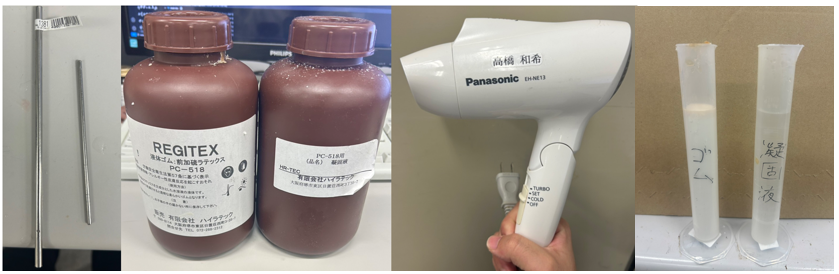
\includegraphics[scale=0.3]{pic/kigu.PNG}
  \caption{使用器具}
\end{figure}
\begin{figure}[!t]
  \centering  % 図全体を中央に配置
  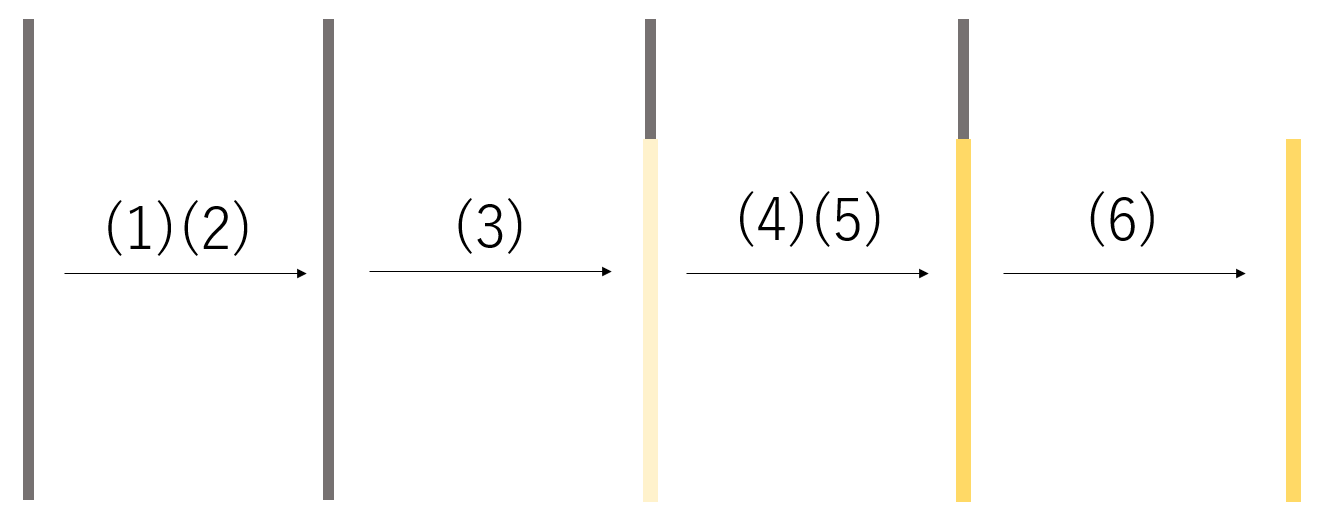
\includegraphics[scale=0.3]{pic/tezyun.PNG}
  \caption{風船の作製手順}
\end{figure}
\begin{figure}[!t]
  \centering  % 図全体を中央に配置
  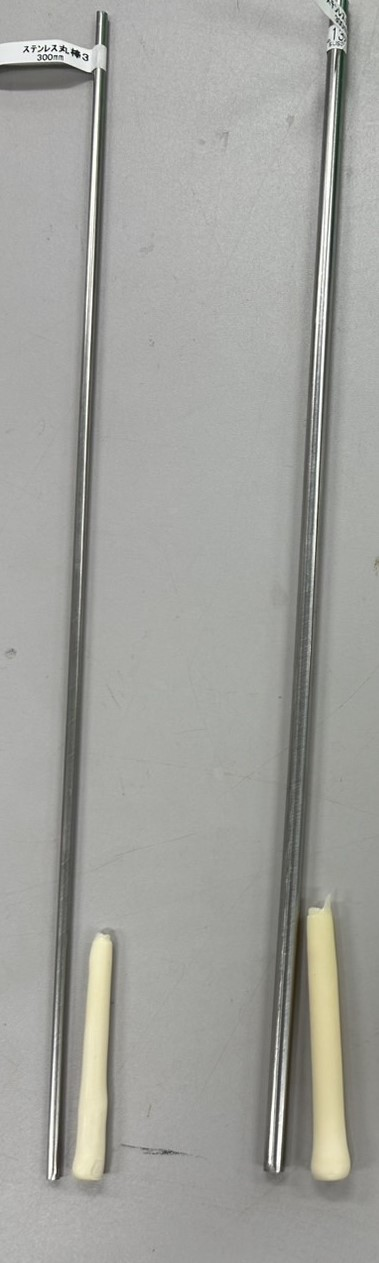
\includegraphics[scale=0.3]{pic/balloon.jpg}
  \caption{作製した風船}
\end{figure}


\subsubsection{問題点の改善}
上記の作製方法で風船を作製するとゴム膜が硬すぎる,ゴム膜の上下で厚さにムラができる問題が生じた.この問題を解決するために以下の方法を行った.
まずゴム膜が硬すぎて膨張させることにかかる印加圧力が多く破裂が起きやすい問題に対して,ゴムと水の比率を変化させることで解決を行った.
初めはREGITEX 液体ゴム(前加硫ラッテクス)の原液のみで作製を行っていた.原液で作製を行うとゴム膜が硬すぎて図5のように破裂してしまった。
そこで実際に売られている風船と同じ比率のゴム60:水40での作製,ゴム膜が形成されるギリギリの比率を調べるためにゴム40:水60での作製を行った。
ゴム60:水40の割合で作製したゴム風船は図6のように破裂をすることなく膨張することが確認できた.一方でゴム40:水60の割合で作製したゴム風船はギリギリゴム膜を形成することができるが空圧を印加するとすぐに膨張が始まり,図7のように
破裂が生じてしまった.次にゴムの上下で厚さに差が出ている問題に対して作製方法の変更で解決を行った.図3を見れば分かるように鉄棒を液体ゴムに浸す時に1回で行っており,上下で液体ゴムに浸っている時間に差が生じてしまっていた.
そこで上と下2回に分けることで解決をした.
作製手順を以下と図8に示す.
\begin{enumerate}
  \item まず初めに鉄棒を凝固液に約5秒浸して取り出す
  \item 取り出した鉄棒を凝固液の水滴がなくなるまでドライヤーで乾かす(水滴が残っているとゴムがダマになってしまいゴム厚に偏りが生じ,破裂が起きやすくなるのでよく乾かす)
  \item 鉄棒を液体ゴムに約5秒浸して取り出す(容器に鉄棒が触れるとゴムの外膜が剥がれるので注意する)
  \item ドライヤーで凝固液の水滴がなくなるまで乾かす
  \item 鉄棒を液体ゴムに約5秒浸して取り出す
  \item 凝固液に約5秒浸して取り出す
  \item 取り出した鉄棒をゴム膜の外側のいろが白色から肌色になるまでドライヤーで乾かす
  \item 3時間程部屋で乾かしたら鉄棒からゴム膜をとる(部屋で放置しすぎるとゴムが硬くなりすぎて鉄棒から取り外すときに割れたり,穴が空きやすくなるので注意する)
\end{enumerate}
\begin{figure}[!t]
  \centering  % 図全体を中央に配置
  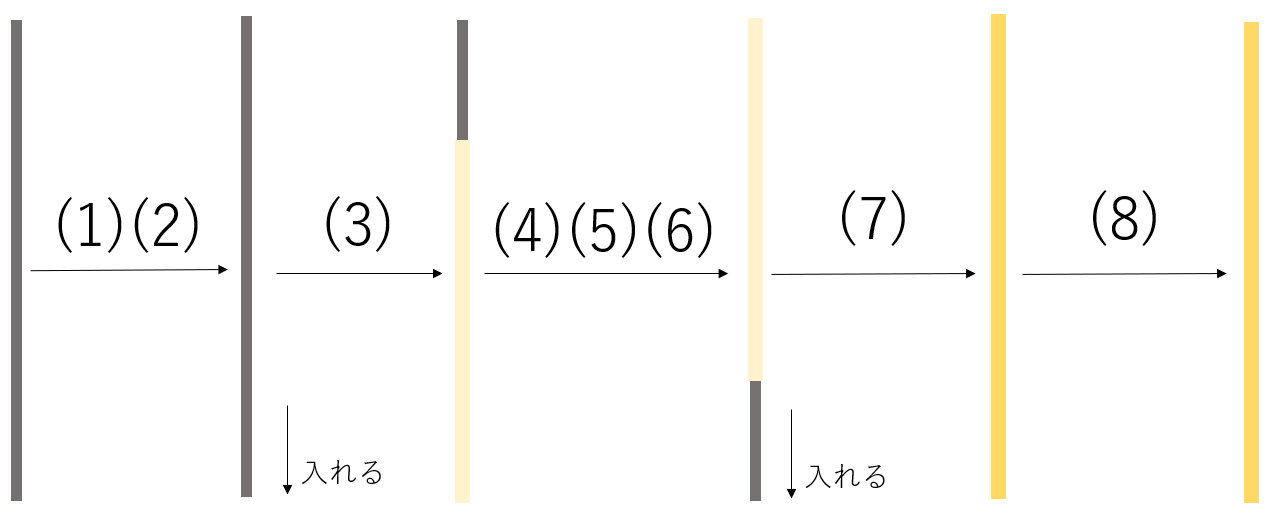
\includegraphics[scale=0.3]{pic/tezyun2.PNG}
  \caption{風船の作製手順}
\end{figure}

\newpage
\subsection{内径5 mmの人工筋肉の作製}
超細径人工筋肉開発の開発に先立ち,まずは内径5 mmの細径空圧筋の作製を行った.作製するにあたって糸を止めるための器具を開発した.
開発した器具の写真を図9,10使用方法について図10に示す.開発した器具は図9のように鉄棒を刺す穴の周りに8つの穴が空いている.中央の穴は鉄棒より少し広い5.3 mm,糸を通す穴は1 mmで設計している.
使用方法としては図10のように鉄棒に器具をはめナイロン糸を通す仕組みになっている.
\begin{figure}[!b]
  \centering  % 図全体を中央に配置
  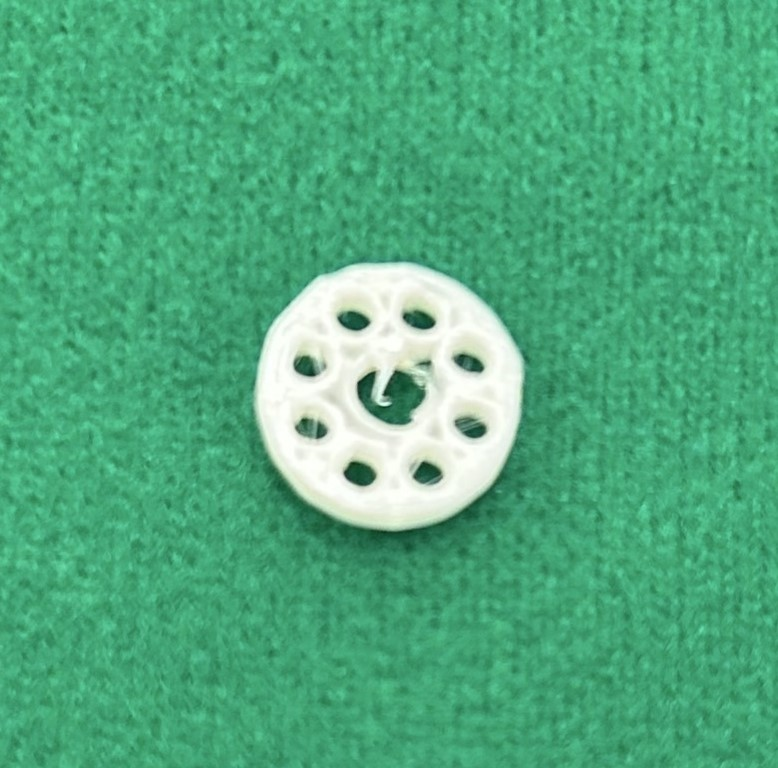
\includegraphics[scale=0.3]{pic/kigu2.jpg}
  \caption{開発した器具}
\end{figure}
\begin{figure}[!b]
  \centering  % 図全体を中央に配置
  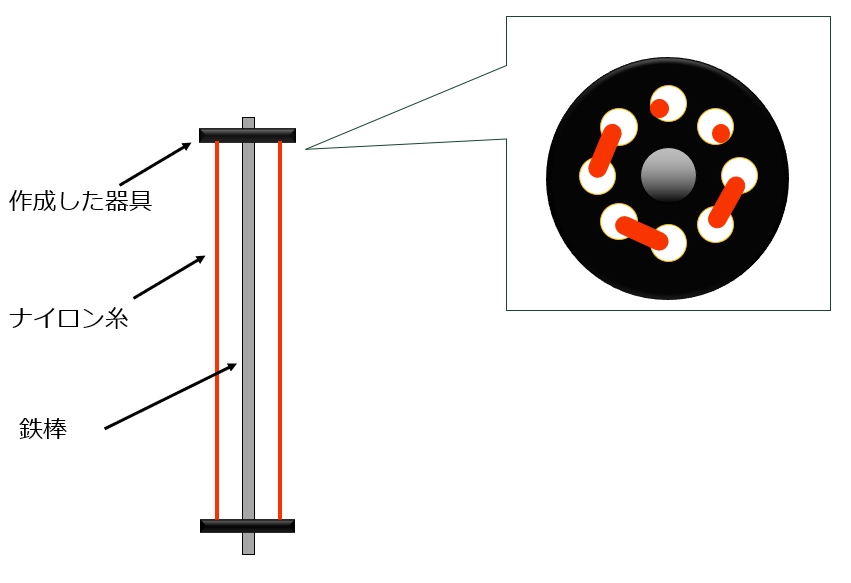
\includegraphics[scale=0.3]{pic/tukau2.PNG}
  \caption{使用方法}
\end{figure}

\begin{figure}[!b]
  \centering  % 図全体を中央に配置
  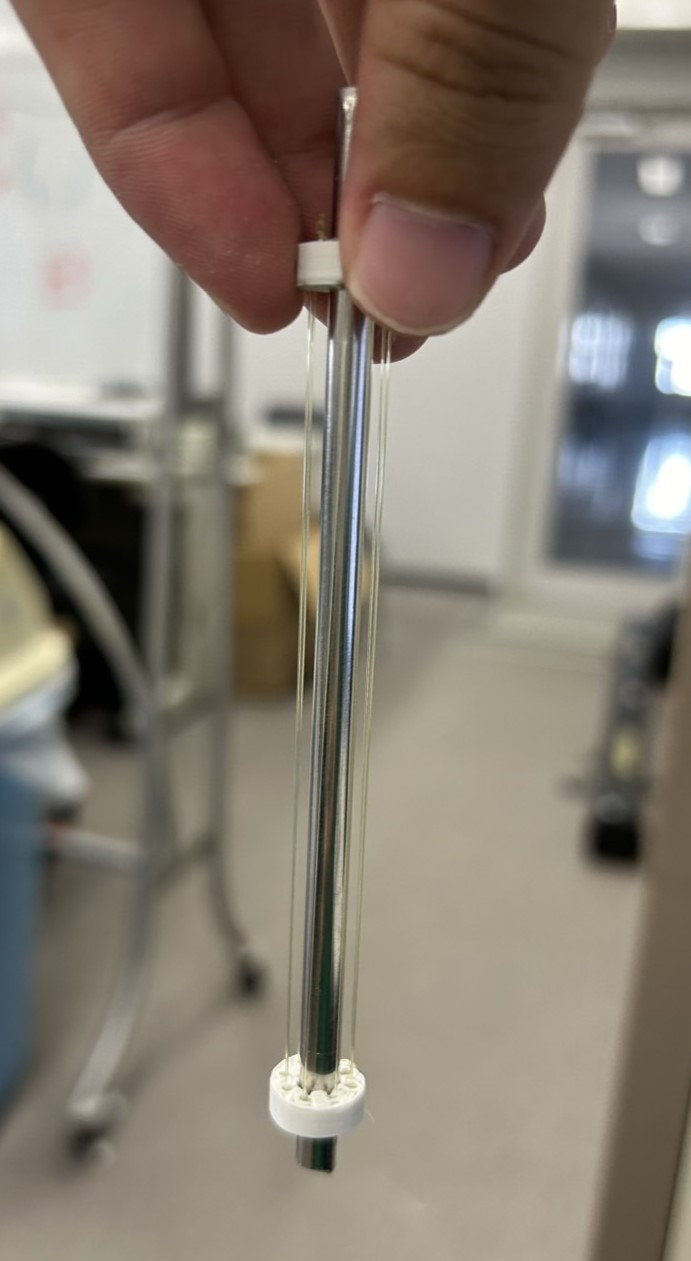
\includegraphics[scale=0.3]{pic/tukau.jpg}
  \caption{使用方法}
\end{figure}
図11に作製に必要な物品,図12,13に作製手順を示す.必要な物品は以下の通りである.
\begin{itemize}
  \item 鉄棒(内径5 mm)
  \item REGITEX 液体ゴム(前加硫ラッテクス) メーカー:有限会社 ハイラテック
  \item PC-518用 凝固液
  \item ドライヤー Panasonic EH-Ne13
  \item 道糸ナイロン 3号 200 m
  \item PPX(瞬間接着剤) メーカー:セメダイン品番:CA-522
  \item PEライン 0.4 mm
\end{itemize}

\begin{enumerate}
  \item まず初めに上記に述べた器具を鉄棒に取り付ける(固定できない場合はPPXを少し塗り,固定する)
  \item ナイロン糸を器具に通す
  \item 凝固液に約5秒浸して取り出す
  \item 凝固液の水滴がなくなるまでドライヤーで乾かす
  \item 液体ゴムに約5秒浸して取り出す
  \item ドライヤーで凝固液の水滴がなくなるまで乾かす
  \item 凝固液に約5秒浸して取り出す
  \item 取り出した鉄棒をゴム膜の外側のいろが白色から肌色になるまでドライヤーで乾かす
  \item 3時間程部屋で乾かしたら鉄棒からゴム膜をとる
\end{enumerate}
以上が本研究で作製した内径5 mmの作製手順である.作製した内径5 mmの人工筋肉を図14に示す.

\subsection{内径3 mmの人工筋肉の作製}
中間発表までの研究によって,内径5 mmの人工筋肉の作製に成功した(図14).そこでさらに細い内径3 mmの人工筋肉の開発に取り組んだ.
開発においては,中間発表までの研究に確立したベースに試行錯誤を行い,最終的に作製手順5にて作製に成功した.以下に各手法の概略と,その過程で生じた問題点について述べる.
\subsubsection{作製方法1}
作製方法1では中間発表の時と同様,鉄棒の周りに糸を張り液体ゴムに漬けることで作製を行った.
作製手順を図15,作製した人工筋肉を図16に示す.
内径が小さくなったことで図16から見て取れるように経糸同士の間隔が狭くなり,互いにくっついてしまう現象が生じた.
これによりゴム膜の幅に偏りが生じ,図17のように空圧印加時に破裂しやすくなってしまった.
\subsubsection{作製方法2}
作製方法3では糸同士の間隔が一定になるように図18のように鉄棒と縦糸の間隔を近づけて作製を行った.作製手順を以下と図19に示す.
\begin{enumerate}
  \item まず初めに器具を取り付ける
  \item ナイロン糸を器具に通す
  \item PEラインを使いナイロン糸を鉄棒に押し付ける
  \item 凝固液に約5秒浸して取り出す
  \item 凝固液の水滴がなくなるまでドライヤーで乾かす
  \item 液体ゴムに約5秒浸して取り出す
  \item ドライヤーで凝固液の水滴がなくなるまで乾かす
  \item 凝固液に約5秒浸して取り出す
  \item 取り出した鉄棒をゴム膜の外側のいろが白色から肌色になるまでドライヤーで乾かす
  \item 3時間程部屋で乾かしたら鉄棒からゴム膜をとる
\end{enumerate}
縦糸がくっつく現象は解決したものの,ゴム部内面に隙間がなくなった結果,図20のように内面側から縦糸が抜けてしまう問題が新たに発生し,軸方向への膨張を抑制することができなかった.
\subsubsection{作製手順3}
作製方法3では糸が簡単に取れなくなるように鉄棒にゴム膜を作り,その上に糸を押し付けて固定し作製を行った.
作製手順を以下と図21に示す.
\begin{enumerate}
  \item 凝固液に約5秒浸して取り出す
  \item 凝固液の水滴がなくなるまでドライヤーで乾かす
  \item 液体ゴムに約2秒浸して取り出す
  \item 凝固液に約5秒浸して取り出す
  \item 凝固液の水滴がなくなるまでドライヤーで乾かす
  \item 液体ゴムに約2秒浸して取り出す
  \item 凝固液に約5秒浸して取り出す
  \item 凝固液の水滴がなくなるまでドライヤーで乾かす
  \item 器具を取り付ける
  \item ナイロン糸を器具に通す
  \item PEラインを使いナイロン糸をゴム膜に押し付ける
  \item 凝固液に約5秒浸して取り出す
  \item 凝固液の水滴がなくなるまでドライヤーで乾かす
  \item 液体ゴムに約5秒浸して取り出す
  \item ドライヤーで凝固液の水滴がなくなるまで乾かす
  \item 凝固液に約5秒浸して取り出す
  \item 取り出した鉄棒をゴム膜の外側のいろが白色から肌色になるまでドライヤーで乾かす
  \item 3時間程部屋で乾かしたら鉄棒からゴム膜をとる
\end{enumerate}
 


